{\fontsize{12pt}{22pt} \textbf{Principal component Analysis}\par}

\vspace{5mm}

The PCA's objective is to get an approximation of data in a \textbf{low} dimensional space. \\

\underline{Inertia} \\

Inertia $I_M = \Sigma_{i=1}^n p_i ||x_i - g||_M^2$ \\

where $g^T = (\bar{x}^{(1)},...,\bar{x}^{(p)})$ also called the \textit{gravity center}. \\

--> The inertia is thus the weighted average of the squared distance of each observation with the gravity center. \\

--> $p_i$ is the weight given to each observation. Most of the times, $p_i = \frac{1}{n}$ (every observation contributes equally to the analysis) \\

-->  the distance $||.||$ depends on the choosen metric $M$ \\

If the data are centered:
$$I_M = \Sigma_{i=1}^n p_i x_i^T M x_i$$

Since $I_M \in \mathbb{R}$:
$$I_M = Tr(\Sigma_{i=1}^n p_i x_i^T M x_i)$$

Thanks to the trace properties:
$$I_M = Tr(\Sigma_{i=1}^n M x_i p_i x_i^T)$$

With $V = Cov(X)$:
$$I_M = Tr(MV)$$

\underline{Projection} \\

In order to represent the data in a low dimensional space, we use projections. \\

The projection should distort the initial space the less as possible, that is:

=> reduce the projection distances as much as possible

=> maximize the average of squared distances between projected points

=> maximize inertia of the projected points \\

In the below figure, maximizing the inertia leads to choosing the projection on the right since d2 > d1.

\begin{center}
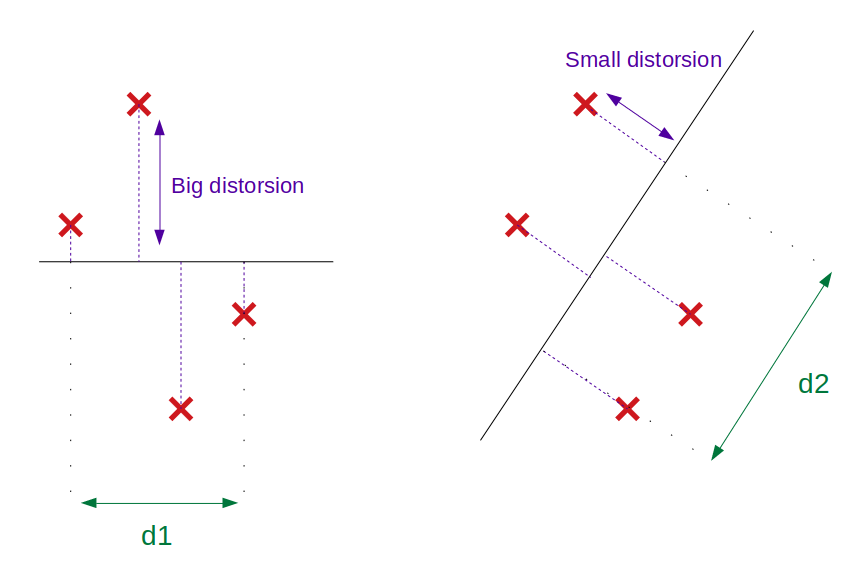
\includegraphics[scale=0.4]{PCA_projections.png}
\end{center}

Let $P$ a projector. $V = Cov(X) = X^TDX$ (with $D$ the weight matrix). The covariance matrix of the projected points is:

$$V_P = (PX)^TD(PX) = (XP^T)^TD(XP^T) = PX^TDXP^T = PVP^T$$ \\

\textit{Note}: a projector $P$ is such that $P^2=P$ and $PM = MP^T$ \\

\underline{Optimisation} \\

As seen previously, the objective is to maximize the inertia. Combining the previous 2 paragraphs, we can express the inertia of projected points:

$$Ip_M = Tr(V_pM) = Tr(PVP^TM)$$

$Tr(PVP^TM) = Tr(PVMP)$ since $PM = MP^T$

$~~~~~~~~~~~~~~~~~~= Tr(VMP^2)$ since $Tr(AB) = Tr(BA)$

$~~~~~~~~~~~~~~~~~~= Tr(VMP)$ since $P^2 = P$ \\

Thus the optimisation problem is:

$$\max~Ip_M = \max~Tr(VMP)$$

The objective is to find the line (in black on above figure) going through $g$ and maximizing the inertia. Let $a$ be a point on this line. We have the following equation:

$$P=a(a'Ma)^{-1}a'M$$

(Indeed we have $P^2=P$ and $PM = MP^T$) \\

$Tr(VMP) = Tr(VMa(a'Ma)^{-1}a'M)$ \\ \\
$~~~~~~~~~~~~~~~= \frac{1}{a'Ma}Tr(VMaa'M)$ \\ \\
$~~~~~~~~~~~~~~~= \frac{Tr(a'MVMa)}{a'Ma}$ \\ \\
$~~~~~~~~~~~~~~~= \frac{a'MVMa}{a'Ma}$ since $a'MVMa$ is a scalar \\

In order to obtain the maximum, we use first order optimal conditions:

$$\frac{d}{da}(\frac{a'MVMa}{a'Ma}) = 0$$

With $\frac{d}{da}(\frac{a'MVMa}{a'Ma}) = \frac{(a'Ma)2MVMa-(a'MVMa)2Ma}{(a'Ma)^2}$, previous equation becomes: \\

$MVMa = (\frac{a'MVMa}{a'Ma})Ma$ \\

Since $\frac{a'MVMa}{a'Ma}$ is a scalar, let's replace it by $\lambda$: \\

$$VMa = \lambda a$$ \\

Based on eigenvalue definition, $\lambda$ is thus the eigenvalue of $VM$. \\

We can thus rewrite the optimization problem:

$$\max~Ip_M = \max~Tr(VMP) = \max~\lambda$$

This final result leads to the theorem: \\

\textbf{The lower dimensional space is given by the eigenvectors associated with the biggest eigenvalues.} \\

Summary of the proof:

Minimization of the distorsion => maximization of the inertia of the projected space => maximization of the covariance matrix's eigenvalues. \\

\underline{Implementation} \\

\lstset{language=Python}
\lstset{frame=lines}
\lstset{caption={PCA}}
\lstset{label={lst:code_direct}}
\lstset{basicstyle=\footnotesize}
\begin{lstlisting}

import numpy as np

def PCA(X , num_components):
 
    # Standardize variables
    X_std = (X - np.mean(X))/np.std(X)
 
    # Compute covariance matrix
    cov_mat = np.cov(X_std , rowvar = False)
 
    # Find eigenvalues and eigenvectors (results of a matrix decomposition)
    eigen_values, eigen_vectors = np.linalg.eigh(cov_mat)
    
    # Sort eigenvalues and eigenvectors
    sorted_index = np.argsort(eigen_values)[::-1]
    sorted_eigenvalue = eigen_values[sorted_index]
    sorted_eigenvectors = eigen_vectors[:,sorted_index]
    
    # Keep eigenvectors associated with highest eigenvalues
    eigenvector_subset = sorted_eigenvectors[:,0:num_components]
    
    # Compute the reduced space
    X_reduced = np.dot(eigenvector_subset.transpose() , X_std.transpose() ).transpose()
    # Note: X_reduced = eigenvector subset = projection of the initial dataset
    
    return X_reduced

\end{lstlisting}

\textit{Note (1)}: standardizing is a good practice before PCA; if not done, variables with high variances will have too much importance. Useful details \href{https://stats.stackexchange.com/questions/53/pca-on-correlation-or-covariance}{here} and \href{https://stats.stackexchange.com/questions/69157/why-do-we-need-to-normalize-data-before-principal-component-analysis-pca?noredirect=1&lq=1}{here}.\\

\textit{Note (2)}: the eigenvectors represent the components (or directions) for the reduced space, whereas the eigenvalues represent the magnitudes for the directions.

\vspace{5mm}